\documentclass{article}
\usepackage[utf8]{inputenc}





\usepackage{verbatimbox,caption,float,lipsum}
\usepackage{float}
\usepackage{listings}
\usepackage{url}
\usepackage{todonotes}
\usepackage{xcolor}
\usepackage{wrapfig}
\usepackage{amssymb}
\usepackage{amsmath}
\usepackage{rotating}
\usepackage[export]{adjustbox}

\newcommand{\ninanotes}[1]{{\color{red} #1}}
\newcommand{\mytodonswer}[1]{{\color{brown} #1}}
\newcommand{\plan}[1]{{\colorbox{cyan} {#1}}}

\newcommand{\KTfourfiveN}{KT$45^n$}
\newfloat{Code}
\captionsetup{Code}


\usepackage[left=3.5cm,right=3.5cm,top=3cm,bottom=3cm]{geometry}  % for page size and margin setting
\usepackage{fancyhdr}
\usepackage{lastpage}
\pagestyle{fancy}

\fancyfoot{}
% \fancyhf{}
% \lhead{Bachelor project}
%\lhead{rettes nederst under opsætning/pakker}
% \rhead{Modal logic}
\rfoot{Page \thepage{} of \pageref{LastPage}}     % page number out of pages
% \lfoot{\today}                                  % gives date 

% \newcommand{\typenaturalnumbers}{\mathbb{N}_0}

% \usepackage{natbib}

\title{Bachelor report:Using modal logic and compact data representations to solve the Hanabi card game}
\author{Christoffer Danborg Irvall (s174256) }
\date{\today}

\begin{document}

% \ninanotes{
% The form and content of a report depend on a number of things:
% \begin{itemize}
% \item The subject/problem the report deals with.
% \item The role of the author (observer, solver, advisor).
% \item The report can be an instruction manual, a maintenance manual, a guide to repeat a process, etc.
% \item The target audience (level of pre-knowledge, is shallow or deep information required).
% \item Are there different target groups needing different information?
% \item Physical restrictions (size, media used, etc).
% \end{itemize}

% \mytodonswer{
% 	\begin{itemize}
% \item Hanabi complexity, optimization and zig
% \item Solver
% \item Design and implementation decisions
% \item The level of preknowledge should be basic computerscience knowledge, basic algorithms, basic compiler knowledge.
% \item no, just CS professors
% \item 20 pages it seems like :)
% 	\end{itemize}

% }

% What to document?:
% \begin{itemize}
% 	\item What is the problem to be solved?
% 	\item Is the problem specified well enough? Otherwise find a sound,
% unambiguous definition.
% \item What is needed to solve the problem?
% \item How is the solution structured?
% \item How is the solution implemented?
% \item What impact will the solution have on whom?
% \end{itemize}

% Problemanalysis
% \begin{itemize}
% \item Check whether the given problem description is clear and the goal is
% well-defined and unambiguous.
% \item Make a problem description which meets these requirements. Have the
% reader in mind, not only the writers.
% \item If needed, invent your own terms to make the description clear, BUT
% describe them to the reader (e.g., in a glossary), not just use them.
% When the original description is vague, this requires a drop in
% abstraction when concretising.
% \item In the same way formulate the goal(s) and the conditions when a goal is
% reached.
% \end{itemize}
% }

% \maketitle
% {\centering
% {
% 	\large
% Bachelor project advisor: Nina Gierasimczuk
% }
% }
\begin{titlepage} % Suppresses displaying the page number on the title page and the subsequent page counts as page 1
	\newcommand{\HRule}{\rule{\linewidth}{0.5mm}} % Defines a new command for horizontal lines, change thickness here
	
	\center % Centre everything on the page
	%------------------------------------------------
	%	READ ME
	%------------------------------------------------
	   
	    %This version of the title page contains both signatures and pictures of participants, this version is best suited for larger reports and or projects. 
	
	%------------------------------------------------
	%	Headings
	%------------------------------------------------
	
	\textsc{\LARGE Danmarks Tekniske Universitet}\\[1.5cm] % Main heading such as the name of your university/college
	
    
\includegraphics[scale=0.15]{images/DTULogo.png}\\
	%\textsc{\Large Major Heading}\\[0.5cm] % Major heading such as course name
	
	%\textsc{\large Minor Heading}\\[0.5cm] % Minor heading such as course title
	
	%------------------------------------------------
	%	Title
	%------------------------------------------------
	
	\HRule\\[0.5cm]
	
	{\huge\bfseries Making self-playable agents for the Hanabi card game using Dynamic Epistemic Logic, compact data representation and a rule-based strategy}\\[0.4cm] % Title of your document

	\HRule\\[0.5cm]
	% \textsc{\Large Danmarks Tekniske Universitet}\\[0.5cm] % Major heading such as course name
	
	 \textsc{\Large Bachelor report}\\[1cm] % Minor heading such as course title
	
	%------------------------------------------------
	%	Author(s)
	%------------------------------------------------
    \begin{minipage}{0.7\textwidth}
		\begin{flushleft}
            \centering
            \large
            By: Christoffer Danborg Irvall (s174256) \\ [0.2cm]
            

	    Advisor: Nina Gierasimczuk \\
                        
		\end{flushleft}
	\end{minipage} 
    \\[1cm]
    \vfill \vfill



	%------------------------------------------------
	%	Date
	%------------------------------------------------
	
	\vfill\vfill\vfill % Position the date 3/4 down the remaining page
	
	% {\large\today} % Date, change the \today to a set date if you want to be precise
	
	\vfill % Push the date up 1/4 of the remaining page
	
\end{titlepage}

\newpage
\tableofcontents
\section{Introduction}

Hanabi (meaning \emph{fireworks} in Japanese) is a cooperative card-game designed by Antoine Bauza \cite{BGGHanabi}. 
In the game each player has a set of cards in their hand and the players must cooperate in order to play the cards in a specific sequence to achieve the highest possible score of 25 points.
The main obstacle for the players is that a player cannot see their own hand, but can see the other players' hands. 
Despite this limitation each player must play cards from their own hand and the only way in which they can know which card to play is based on specific hints and counting the cards. 
Since what a player can know for sure is quite restricted, each player, in practice, will have to guess the intention of the other player i.e. have a theory of mind. 
Since it is a game with imperfect knowledge, as well as good strategies have some theory-of-mind in place, it has sparked some notable interest in the AI research \cite{DeepmindAndOthers}. 

In this thesis I will focus on \emph{self-play} i.e. only AI agents will have to cooperate in order to get as high a score as possible, as opposed to \emph{cross-play} where some or most of the players are actually humans that try to cooperate with one or more agents.  

Solutions to the problem includes hat-guessing strategies \cite{CoxEtAl2015}, Cox et al develop two strategies, one for recommending moves to other players, denoted recommendation strategy, and one for increasing other players' knowledge of what cards they currently hold, denoted information strategy. 
A hat-guessing strategy utilizes the fact that any legal move in the game can be interpreted as an encoding about some information or recommendation.
This encoding can then be decoded by each individual, giving rise to some information or recommended action. 
Such strategies have proven effective for Hanabi, with \cite{CoxEtAl2015} getting an average of $23.00$ points for their recommendation strategy and $24.68$ points for their information strategy. 
Looking into these strategies in detail, I reckon that these strategies are not only effective, but also efficient, because it is a very small amount of data each agent has to keep track of, and deducing the encoding and updating auxiliary data seems quite trivial for a computer.
Other solutions utilize Dynamic Epistemic Logic \cite{EgerAndMartens17}, that can very declaratively specify goals and try to find shortest paths in order to satisfy these goals. 
There are also machine-learning oriented solutions to this problem \cite{hu2021otherplay}, that nowadays seem to be on-par with the rule-based ones achieving average score of $24.09$.

In this thesis I will describe my solution based on principles of Dynamic Epistemic Logic, with emphasis on knowledge about ones hand, in order to make a group of agents work together and attempt to score as many points as possible in Hanabi. 

The choice of implementation language is Zig \cite{Ziglang}, a new C-like language, which offers a lot of low-level control to the programmer, making it possible to create some highly-optimal data-structures as well as some nitty-gritty optimizations possible at the bit-level.



\subsection{Instructions on how to run the code}
\todo[inline]{later}
You will need the Zig compiler in order to run the code. Navigate to this page \url{https://ziglang.org/download/} and download a version 0.10.1, matching your computer's architecture.

Once you have the compiler, you can navigate to the folder {\tt AgentsAndGameSimulator} and run the command: {\tt \$ zig build run-agents -Drelease-fast=true}

The {\tt Drelease-fast=true} is optional, but makes sure it is compiled with optimizations.



\subsection{Hanabi setup and rules}
For completion I will give a short summary of the rules in Hanabi, which will also serve as terminology later on in the report.

Hanabi consists of a \emph{Deck} of 50 cards, 4 \emph{black tokens}, 8 \emph{blue tokens}.  
Of the cards there are 5 \emph{suits} and 5 \emph{values}. 
The suits are red, green, blue, white, yellow. 
The values are 1 through 5. 
For each suit there is three cards of value 1, two cards of value 2, two cards of value 3, two cards of value 4 and one card of value 5.
The number of cards in each player's hand depends on the number of players. If there are 3 players or less, they will have 5 cards each. 
Otherwise they will have 4 cards each.

The goal of the game is to play add as many cards as possible to the \emph{colour piles}. 
There are 5 colour piles, one for each suit. 
You gain a point for each card in the colour piles, with a maximum of 25 points.

A player can spent her turn on one of the following actions

\begin{itemize}
\item Play a card
\item Give a hint
\item Discard a card
\end{itemize}

\paragraph{Playing}
When playing a card you attempt to add a card to one of the colour piles.
You can add a card $c$ to a pile of identical suit $p$ if either, 

\begin{itemize}	
\item $p$ is an empty colour pile and $c$ is of value 1.
\item $p$ is non-empty and $c$'s value is exactly one greater than the current card on top of the pile.
\end{itemize}

If a card does not add to a colour pile then it is put in the \emph{discard pile} and then the game removes 1 black token. 
If there are no black tokens the game ends immediately.  

\paragraph{Hinting}
If a player chooses to hint, he can hint any other player. 
Hints are restricted, so you can either hint about cards matching a suit or cards matching a value. 
Imagine a hand of following configuration: ((red,1),(blue,3),(red,2),(yellow,3)), each having respective indices 0 through 3. 
Then if you hint "cards of value 3", then you have to give the positions of both (blue,3) and (yellow,3) i.e. index 1 and 3. 
And if you give the hint "cards of red suit" then you have to give the position of both (red,1) and (red,2) i.e. index 0 and 2. 
You cannot give an "empty hint" like "there are no green cards".

When giving a hint it removes 1 blue token, if you cannot do that, you cannot give the hint.

\paragraph{Discarding}
A player can discard any card on their hand, and it will result in the card going in the discard pile and it adds 1 blue token (and can only be done if there are less than 8 blue tokens left).

\paragraph{End of the game}
The game ends immediately if there are no black tokens left. 
The game also ends if the last card from the deck has been drawn, in which case every player can play an additional round (including the player who drew the last card) and then the game ends.

After the game ends the score is decided by counting how many cards there is in the colour piles.





\section{Problem analysis}
\todo{
\begin{itemize}
\item Coarse problem analysis Describing the problem and goals in more
detail, briefly analysing the challenges, pointing out possible solutions.
\item Problem specification and analysis Detailed specification of the
problem (and goals). This might need to introduce new notation in order
to arrive at a precise description. If relevant, make state-of-the-art
solutions precise and compare.
\item Goals and success criteria Describe the goals and when a goal is
reached.
\end{itemize}
}

\section{Design}
\ninanotes{
\begin{itemize}
\item Design
\item How is the solution constructed, on which design elements?
\item Which components does the solution consist of?
\item Which technologies, tools or packages are used?
\item Discuss alternatives and motivate your choice.
\end{itemize}
}
\newcommand{\POVModel}{\mathcal{M}}

% \subsection{Representing a card and deck compactly}
% Since a single card cannot take more one of 25 different, then enumerating each card, a single Card type needs 5 bits in order to reperesent a value.





Given the constraints on time and space, it would be nice to have a quite compact representation of each world, furthermore, given that query algorithms will go through most (if not all) of the possible worlds, iterating though the possible worlds should be fast. A fast way to iterate through elements is to make sure that each element is small as well as contiguous in order to make use of the CPUs caching system the most, i.e. small elements in a contiguous data structure which guarantees good spatial locality.


\subsection{Formalizing accessing in a model} \label{sec:model-access}
In order to get good spatial locality I want to explain how to take the model from section \ref{sec:description-of-how-modal-logic-is_applied} and describe how it might be turned into an array.

In the section \ref{sec:description-of-how-modal-logic-is_applied} I went through the overall approach of generating the worlds from a specific agents POV. In order to specify how such worlds might be accessed, I extend the solution with some notation. Let $\POVModel_p: W \rightarrow P \rightarrow \mathcal{P}(W)$ be the model for the player $p$'s POV. Here the interpretation is that the model takes some fixed scenario $w$ of type $W$, and some player $b$ of type $P$, then we have all the worlds that $p$ cannot rule out that $b$ finds possible, given that $w$ is the case. Of course if $b=p$ then we have the unit set, which is simply $\POVModel_p(w)(p) = \{w\}$. Which also makes sense in the interpretation "given that we fix the world to $w$, then player $p$ can only imagine that $p$'s only possible world is $w$". 

It is clear from the above mapping that this could be encoded using a 3-dimensional array. Where $W$ (the first argument) could be an enumeration of the possible worlds for $p$, and $P$ could be an enumeration of the players, and $\mathcal{P}(W)$ could be an array of possible worlds.



\subsection{Representing the world} \label{sec:representing-a-world}
A world is simply a possible state of the entire game, i.e. everything is specified, including the hands you can't see. A naive approach to representing a world is to take the deck, the discard pile, all of the hands etc. into account. But this approach is definitely more than necessary, since what is in the discard pile and in the color pile, as well as most hands, are information easily accessed by the agents themselves, by checking the current state of affairs. Furthermore I choose not to take order into account in any of the hands or piles, because it would lead to too many combinations (a hand of 4 cards has 25 permutations, assuming that all are unique). What is most interesting to represent is simply then what is uncertain. So in this case it is a player's own hand and the deck. Of course assuming some hand will give an unambigous content of the deck, and vice versa, so it is sufficient to just represent the unknown hand. So a query $\POVModel_p(w)(b)$, will return the set of hands that $p$ cannot rule out that $b$ believes, given that the hand $w$ is the case for $p$.

There are various approaching to representing a hand, I will go through a few I have deviced. 

\begin{enumerate}
\item Represent each card in a sorted order. Called sorted-order representation
\item Enumerate each possible hand. Called Enumeration representation
\item Contingency table inspired set. Called table representation.
\end{enumerate}

In each representation I will go through the number of theoretical bits needed per world as well as what the actual number of bits are if we have to make it directly byte-addressable. The reason I write "theoretical" is due to that most CPU architectures (as well as how Zig compiles code \cite{zigdocspackedstruct}) are byte-addressable. This means that the smallest adressable space is 1 byte on most modern architectures, even if you want to represent something that uses fewer bits. The theoretical number of bits can be reached, but will require some packing of structs or bitmanipulation, and comes with the tradeoff of more CPU cycles spent on bitmasking the value rather than simply accessing it. 


\paragraph{Represent each card in a sorted order}
So firstly we want to look at how small can we get away with representing a card. A card can be one of 25 different instances (5 suits times 5 values), so a minimal representation could enumerate each card and a world be represented by 5 bits (which can represent from 32 different values).
Then if we have a hand of 4 cards, that means we spent $4 \frac{\text{cards}}{\text{hand}} \cdot 5 \frac{\text{bits}}{\text{cards}} = 20 \frac{\text{bits}}{\text{hand}}$. And using the same reasoning we use 25 bits for 5 cards.
Then we can predefine some sorted order of the 25 different instances, and just sort a hand in order to get its set representation.

If each card has to be byte-addressable then it would have to use 1 byte (8 bits), which would then mean that a hand of 4 cards is 24 bits, and a hand of 5 cards is 40 bits.

Pros: Very simple and compact representation. No obvious cons.

\paragraph{Enumerate each possible hand}
If you draw 4 cards blindly from an initial deck of 50 cards, there are 18480 distinct combinations (data from Appendix \ref{appendix:python-distinct-combinations}). If it 5 cards drawn it is 99455. 
Depending on the situation, you could enumerate each possible hand. Then a world need only an integer size large enough to store 18480 or 99455 depending on the case. This is respectively 15 bits and 17 bits.
So this representation is definitely compact. Of course some edge-cases exists, for instance in a 5 player game, when the last card has been drawn, then there can exist both 4 and 5 cards representations at the same time, but that would require bits enough to represent $18480+99455 = 117935 < 2^{17}$ so 17 bits should still be sufficient.

Of course if the representation would have to be byte-addressable in an array, then it would have to spent a whole number of bytes, which is repectively 2 bytes (16 bits) or 3 bytes (24 bits).

Of course this enumeration would only create a mapping from an integer to an actual representation, so we would still have to choose a representation that this integer maps to. Which can be either sorted-order or table representation

Pros: Very compact representation, the enumeration map should only take some constant amount of memory at all times. Even if we assume the worst case, which is using the table representation and enumerating

Cons: Non-trivial to implement. A lot of conversion between values i.e. its hard to work on a world directly without looking it up in a map, so when iterating through a list of possible worlds I will have to look up what that world actually is, this I imagine will substantially slow down the algorithm, although I have not tested it.

\paragraph{Contingency table inspired set}
This representation I stumpled upon when trying to figure out how to generate the possible hands in a fast manner (more on the generation in section \ref{sec:efficient-generation-of-hands}).
Given that instance of a card can at most occur 3 times in a hand (or deck for that matter). Then an array of 25 elements, each element being able to store 0 through 3, will be a sufficient representation. This means that each element in the array need only be 2 bits. So a theoretic use of space is $2 \frac{\text{bits}}{\text{elements}} \cdot 25\text{elements} = 50$ bits. 

If each element has to be byte-addressable then it will have to spent 1 byte per element, in which case $8 \frac{\text{bits}}{\text{elements}} \cdot 25\text{elements} = 200$ bits. Which is a pretty big increase from the theoretical 50 bits.  

Pros: Very direct set representation of the cards, can even be used for the piles and deck. 

Cons: Spents a lot more bits than strictly necessary to represent a world.


\subsubsection{Choosing a representation}
All representations have a convincing set of of tradeoffs. I decided to go with the table representation, since it is very generalizable for other aspects of the game (i.e. can be used to represent decks, piles etc.), as well as easy to work on directly, as well as generate, see section \ref{sec:efficient-generation-of-hands}. 
But the other representations should definitely be kept in mind if memory proves to be a problem in practice.


\subsection{Generating hands in an efficient way} \label{sec:efficient-generation-of-hands}
Using the methods described in math.stackexchange posts "Efficient algorithm to find all unique combinations of set given duplicates" \cite{HardmathcontigencyTablePost} and \cite{GCabrecursiveGenerationPost}, I was able to design a good generation method for the hands. 
The main idea is that we represent the hands we want to generate in a contingency table, where we have some pool to take from. So a case with handsize set to 0 and the pool being the initial deck will be Figure \ref{fig:hand-pool-table} (of course in a practical game, you would know something about the other hands and the discard pile etc. so the pool would be less than the initial deck). Then the problem is to generate all such contingency tables, such that the sum of the hand is $k$ (usually 4 or 5), and the column sums stay the same, for example see Figure \ref{fig:hand-pool-table-with-hand}.

\begin{figure}
	\centering
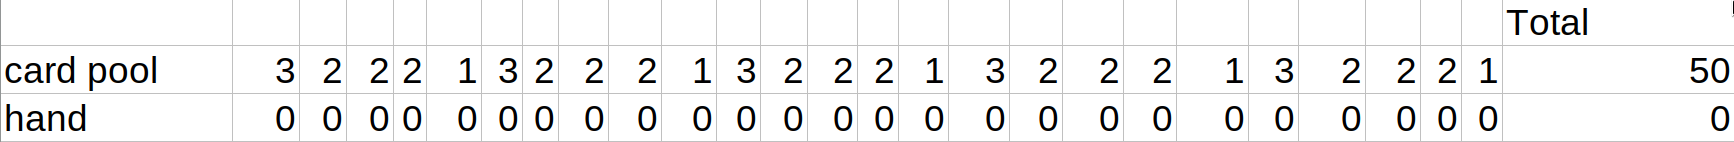
\includegraphics[width=13cm,frame]{images/contigency_table.png}
	\caption{Contingency table with handsize set to 0}
	\label{fig:hand-pool-table}
\end{figure}


\begin{figure}
	\centering
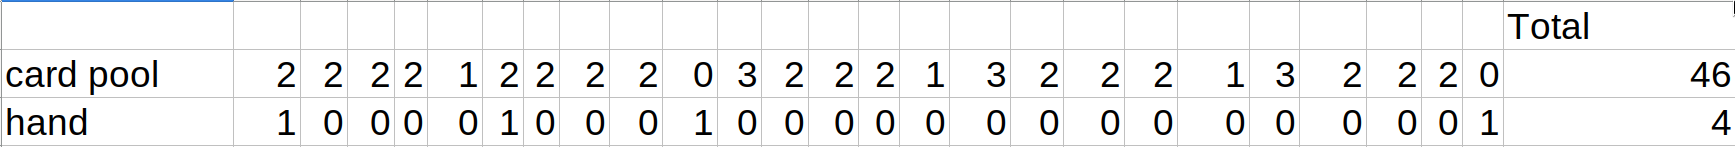
\includegraphics[width=13cm,frame]{images/contigency_table_with_hand.png}
	\caption{Contingency table with handsize set to 4}
	\label{fig:hand-pool-table-with-hand}
\end{figure}

Both the card pool and the hand can be represented by using the table representation described in section \ref{sec:representing-a-world}.

The simplest way to describe how the hand is generated, is to view the hand table entries as digits in an integer (or more mathematically specific, a multi-radix integer), with the leftmost digit being the most significant, and then you create the biggest integer with cross-sum $k$, and subsequently construct the number just below that, still with constraint that the cross-sum must be $k$. So continuing the example with Figure \ref{fig:hand-pool-table}, we can create the "biggest integer" in this way Figure \ref{fig:biggest-integer}. Then the integer just below that is Figure \ref{fig:next-integer}. And continuing with 1s until we get Figure \ref{fig:etc-one}.
Then we decrement the most signficant digit and get Figure \ref{fig:decrement}.

\begin{figure}
	\centering
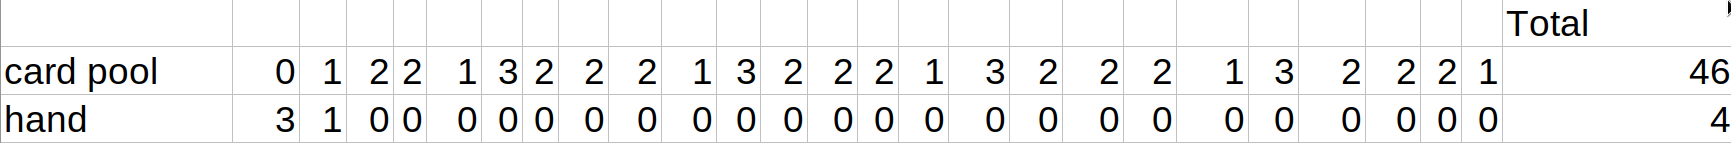
\includegraphics[width=13cm,frame]{images/biggest_integer.png}
	\caption{First generated hand}
	\label{fig:biggest-integer}
\end{figure}

\begin{figure}
	\centering
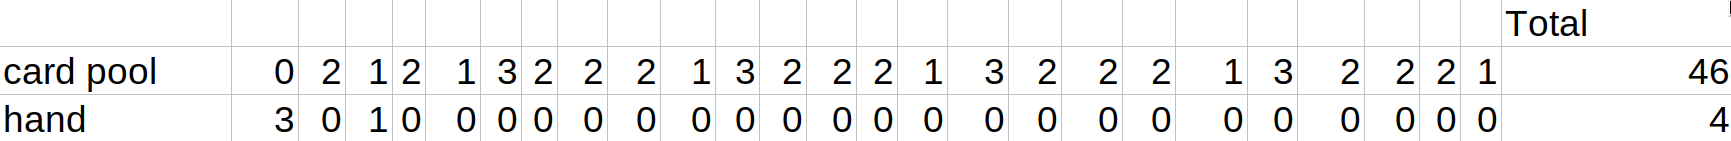
\includegraphics[width=13cm,frame]{images/next-biggest.png}
	\caption{Second generated hand}
	\label{fig:next-integer}
\end{figure}

\begin{figure}
	\centering
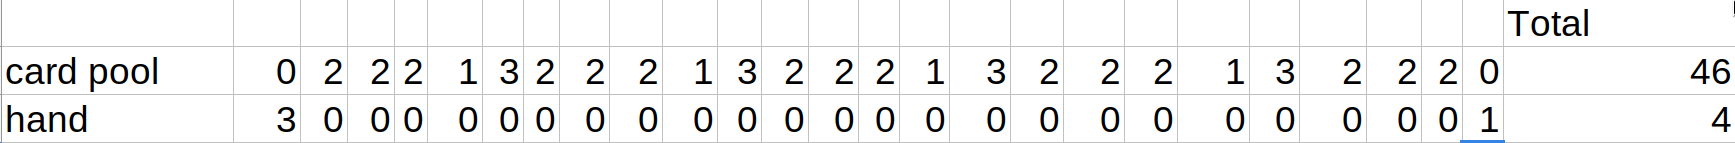
\includegraphics[width=13cm,frame]{images/etc_one.png}
	\caption{The smallest integer containing 3 in the first position}
	\label{fig:etc-one}
\end{figure}


\begin{figure}
	\centering
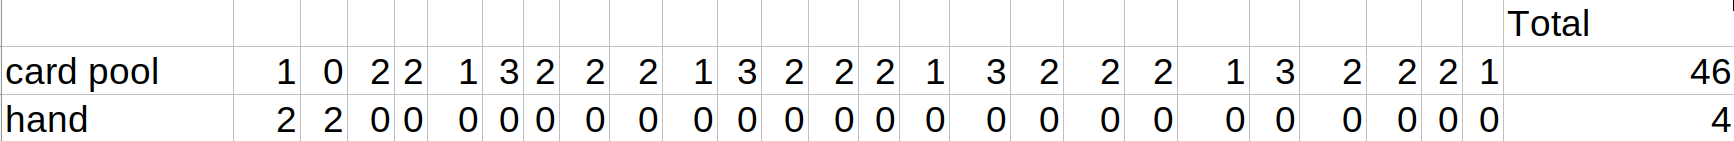
\includegraphics[width=13cm,frame]{images/decrement.png}
	\caption{The biggest integer containing 2 in the first position}
	\label{fig:decrement}
\end{figure}


A more formalized algorithmic approach will be described in the implementation chapter.


\subsection{How should an agent play?} \label{sec:how-should-an-agent-play}

How an agent should play based on its knowledge in its DEL model is heavily inspired by \cite{CoxEtAl2015}, specifically the "information strategy". 
In it they distinguish between \emph{public and private information}. Where public information is what everybody knows, and everybody knows that everybody knows that etc. And private information, is what an agent individually knows based on the other players hands. This can be compared to DEL where public information is what the model guarantees is common knowledge, and private information is simply queries that holds true for all possible worlds from that agents POV.

In my solution I will only look at private information, but it is an interesting problem to see how one can adapt the model I have described into something that can answer common knowledge queries, especially given that \cite{CoxEtAl2015} information strategy makes use of common knowledge.

In order to decide what an agent should do in a specific situation, I borrow terminology from \cite{CoxEtAl2015} again. So given a hand, which is a ordered set of known or unknown cards, how does an agent know what card to play?


% In order to decide what an agent should do in a specific situation, I borrow terminology from \cite{CoxEtAl2015} again. So given a hand, which is a ordered set of known or unknown cards

% However the private information my agents got is not the tables defined in \cite{CoxEtAl2015}, but the DEL model described in section \ref{sec:model-access}. The action algorithm for the information strategy is as follows (most of it cited directly from \cite{CoxEtAl2015}):

% Adapting \cite{CoxEtAl2015} information strategy to the model I have described is pretty straight-forward. 

Firstly I will have to decide \emph{when} a card should be played, discarded etc. Here I use the action algorithm from \cite{CoxEtAl2015}:
\begin{enumerate}
	\item Play the playable card with lowest index.
	\item If there are less than 5 cards in the discard pile, discard the dead card with lowest index.
	\item If there are hint tokens available, give a hint.
	\item Discard the dead card with lowest index.
	\item If a card in the player’s hand is the same as another card in any player’s hand, i.e.,it is a duplicate, discard that card.
	\item Discard the dispensable card with lowest index.
	\item Discard index 0.
\end{enumerate}

Here implicitly "playable card", "dispensible card", "dead card", "it is a duplicate", are epistemic queries on the $\POVModel_p$ for the current playing player $p$'s hand. So how would an agent go about trying to decide whether a card is playable, discardable, dead, a duplicate or dispensible? Let's denote each of these the cards \emph{actionable states}.

I define the actionable states is as follows (also based on \cite{CoxEtAl2015}):
\begin{itemize}
	\item Playable: If it is able to be played in the current game state.
	\item Dead: If the card has already been played and is not needed anymore.
	\item Dispensible: If the card could be played at some point (now or in the future), but there is at least one more of the same card left.
	\item Duplicate: There exists duplicate in another players hand.
\end{itemize}

The problem with deciding actionable states for the cards is that we have stored each world as a set, and since a set ignores order of the cards, then even if we find hands with several actionable states in the model, we still have to find a mapping between the set and the ordered list that is the concrete hand that the agent is playing with.
So for the agent's POV, the hand the player has can be viewed as an ordered list of what is hinted about the agent's cards. What is known about a card can be denoted by a pair: its suit, and its value. 

As an example: If I have the hand ((red,1),(blue,3),(red,2),(yellow,3)), and the current state of the game I have only my red cards hinted, then the ordered list $o_{hints}$ is (red,unknown),(unknown,unknown),(red,unknown),(unknown,unknown).

In order to create the mapping from a set in a world to an ordered list that matches the hand indices, we have to take the hints given to player $p$ into account.
So given an unknown hand for player $p$ specified with the ordered list of hints $o_{hints}$, and the model $\POVModel_p$ we have to decide what possible actionable states is in each card. 

For each possible world for $p$, there is a specific hand for $p$, denoted $h_{specific}$. Since each hand is stored as a set, we have to use the hints $o_{hints}$ to figure out how the set should be mapped to ordered list. How this can be done is to make $h_{specific}$ into any ordered list $o_{specific}$ and subsequently take all permutations of $o_{specific}$ and see which ones matches the $h_{hints}$. If it is possible to find any permutation that is non-contradictory with $o_{hints}$ then we can decide the actionable states for each card given by $h_{specific}$.

Continuing the previous example. We might have the set \[h_{specific} = \{(green,1),(red,5),(green,2),(red,1)\}\]
Turning this into an ordered list 
\[o_{specific} = ((green,1),(red,5),(green,2),(red,1))\]
we see that there are 4 permutation that matches $o_{hints}$:

\[o_{1} = ((red,5),(green,1),(red,1),(green,2))\]
\[o_{2} = ((red,1),(green,1),(red,5),(green,2))\]
\[o_{3} = ((red,5),(green,2),(red,1),(green,1))\]
\[o_{4} = ((red,1),(green,2),(red,5),(green,1))\]

Then for each permutation we can decide the actionable states of each card, based on the permutation and the current state of the game. For instance, let us assume that the red color pile in the current state of the game has a 4 on top. This means that the card in position 0 can both be playable (if it is a (red,5)). But it is also unplayable (i.e. if it is a (red,1)). Since we can't know for sure based on our knowledge, then we cannot perform action 1 in the action algorithm.



\todo[inline]{probably better to mention in implementation} 
Generating permutations can be done using Heap's algorithm \cite{wiki:heapsalgorithm}, which seem to be fast and not need that much extra data in order to compute the permutations. 

\subsection{Removing other players possible worlds based on their hints} \label{sec:design:removing-worlds-based-on-hints}
When a player $p$ has their model $\POVModel_p$, then for some player $b$, there are some possible worlds which player $p$ cannot rule out are possible for $b$, therefore they are generated as well. But if this generation is only based on the cards revealed then there will be some possible worlds which conflict with the hints given to $b$, therefore we can also go through all possible worlds for $b$ and remove any that are in conflict with their hints. This can be done in much the same way as described in section \ref{sec:how-should-an-agent-play}, where we use permutations of a possible world to see if any permutation matches the hints.


\section{Implementation}

\subsection{Going through all permutations}
In sections \ref{sec:how-should-an-agent-play} and \ref{sec:design:removing-worlds-based-on-hints}, I described how to respectively how an agent might know what to do with their cards and how to remove worlds based on hints. A crucial aspect of both of these procedures is that we need a permutation generation method.
Generating permutations can be done using Heap's algorithm \cite{wiki:heapsalgorithm}, which seem to be fast and not need that much data in order to compute the permutations. If there are $k$ objects that you want to find the permutations of, you only need to maintain some auxiliary arrays of size $O(k)$. My implementation is in "{\tt src/multi\_agent\_solvers/PermutationIterator.zig}". 


\subsection{Generating distinct combinations of size $k$} \label{implementation:sec:generating-distinct-combinations}
Continuing the section \ref{sec:efficient-generation-of-hands}, I wanted to generate all distinct combinations from a set of elements (where some are duplicates). The approach I found is best described with the pseudo-code in Code listing \ref{code:distinct-combinations}. 

It takes a array {\tt  taken\_into\_account} in which initially all elements are 0, which, when filled with {\tt cross\_sum} number of elements will represent a hand. {\tt distinct\_pool} which represents the set from which the $k$ distinct combinations will be generated from. {\tt sum\_array} is a suffix-sum array of the initial {\tt distinct\_pool}. {\tt cross\_sum} which is initially the same as $k$. {\tt current\_id} is which element is being considered to be added to the hand and finally {\tt accumulator} stores all the distinct combinations.

As an example, for generating all distinct combinations of $k=4$ from the card-pool array in Figure \ref{fig:hand-pool-table}. Then the {\tt distinct\_pool} array would be equivalent to the card pool row (except for the "Total" column). And the suffix-sum array {\tt sum\_array} would be
\[
[50, 47, 45, 43, 41, 40, 37, 35, 33, 31, 30, 27, 25, 23, 21, 20, 17, 15, 13, 11, 10, 7, 5, 3, 1, 0]
\]

The suffix-sum array is an optimization, that I found gave notable speed up when implementing this generation method.



\begin{verbbox}
function distinct_combinations(
 taken_into_account: integer array consisting of 25 elements, 
 distinct_pool: integer array consisting of 25 elements, 
 sum_array: integer array consisting of 25+1 elements, 
 cross_sum: integer, 
 current_id: index, 
 accumulator: growable array) {
    if (cross_sum == 0) {
        acc.append(taken_into_account) 
        taken_into_account[current_id] = 0;
        return;
    }

    take = math.min(distinct_pool[current_id], k); 

    for(int i = 0; i < take + 1; i = i + 1){
            taken_into_account[current_id] = take - i;
            if (sum_array[current_id + 1] < k - (take - i)) {
                taken_into_account[current_id] = 0;
                return;
            }
            distinct_combinations(taken_into_account, 
	     distinct_pool, 
	     sum_array, 
	     cross_sum - (take - i), 
	     current_id + 1, acc);
     }
     taken_into_account[current_id] = 0;
}
\end{verbbox}
{\centering
\fbox{\theverbbox}
\captionof{Code}{Pseudo code for the hand-generation method. It is assumed that arrays are taken by reference and integer/indices are called via copy}\par
\label{code:distinct-combinations}
}



\subsection{Representing the world}
I mentioned that I picked the table representation from the different choices I had (see section \ref{sec:representing-a-world}), but I was not aware, at the time, of how byte-addressability would affect the actual space, so I was surprised that the space was filled up so quickly. There are ways to mitigate these problems of space by using porting the current encoding of 25 bytes, to make a packed array that uses bit manipulation in order to achieve this \footnote{Zig has this in its library called packed int array \cite{zigpackedintarr}}. Due to time left to finish up this product I chose to have only 1 agent with 1 model at a time, so that the agents in total do not use too much memory.

\subsection{Implementing the board game}
I also implemented the board game, simply referred to as the Game struct (in file "{\tt src/hanabi\_board\_game.zig}) in order for the agents to interact with the game. The board game keeps track on who is the current player and has some simple methods that the agents can use when they want to make a move:

\begin{itemize}
	\item {\tt play(index)}
	\item {\tt discard(index)}
	\item {\tt hint\_color(color, index\_of\_player) }
	\item {\tt hint\_value(value, index\_of\_player) }
\end{itemize}
In order to simplify the implementation of the board game, I simply let it crash if a agent does something that is illegal. (Like giving an index that is out of bounds, or hinting a colour not on the hinted players hand).


\subsection{Agents}
The logical agents in the game are implemented as an Agent struct. See a class diagram on Figure \ref{fig:Agent-class-diagram}.
An Agent has a hand that is represented with {\tt CardWithStates}, here the states refer to each cards actionable states (related to section \ref{sec:how-should-an-agent-play}), but also its hints. It does not see the actual cards. It has a {\tt KripkeStructure} which is its epistemic model. And lastly it has a {\tt CurrentPlayerView} which is the current game that the agent as a player is able to see i.e. it cannot see its own hand, or the contents of the deck. An Agent has a method called {\tt init(...)}, that based on the view and which player it is, is able to generate the entire model, as well as decide what states the {\tt CardWithStates} should be in. After an Agent has been {\tt init}ed it can make a move with the method {\tt make\_move(game)}, which modifies the game based on its {\tt hand}, as well as its view.

\begin{sidewaysfigure}
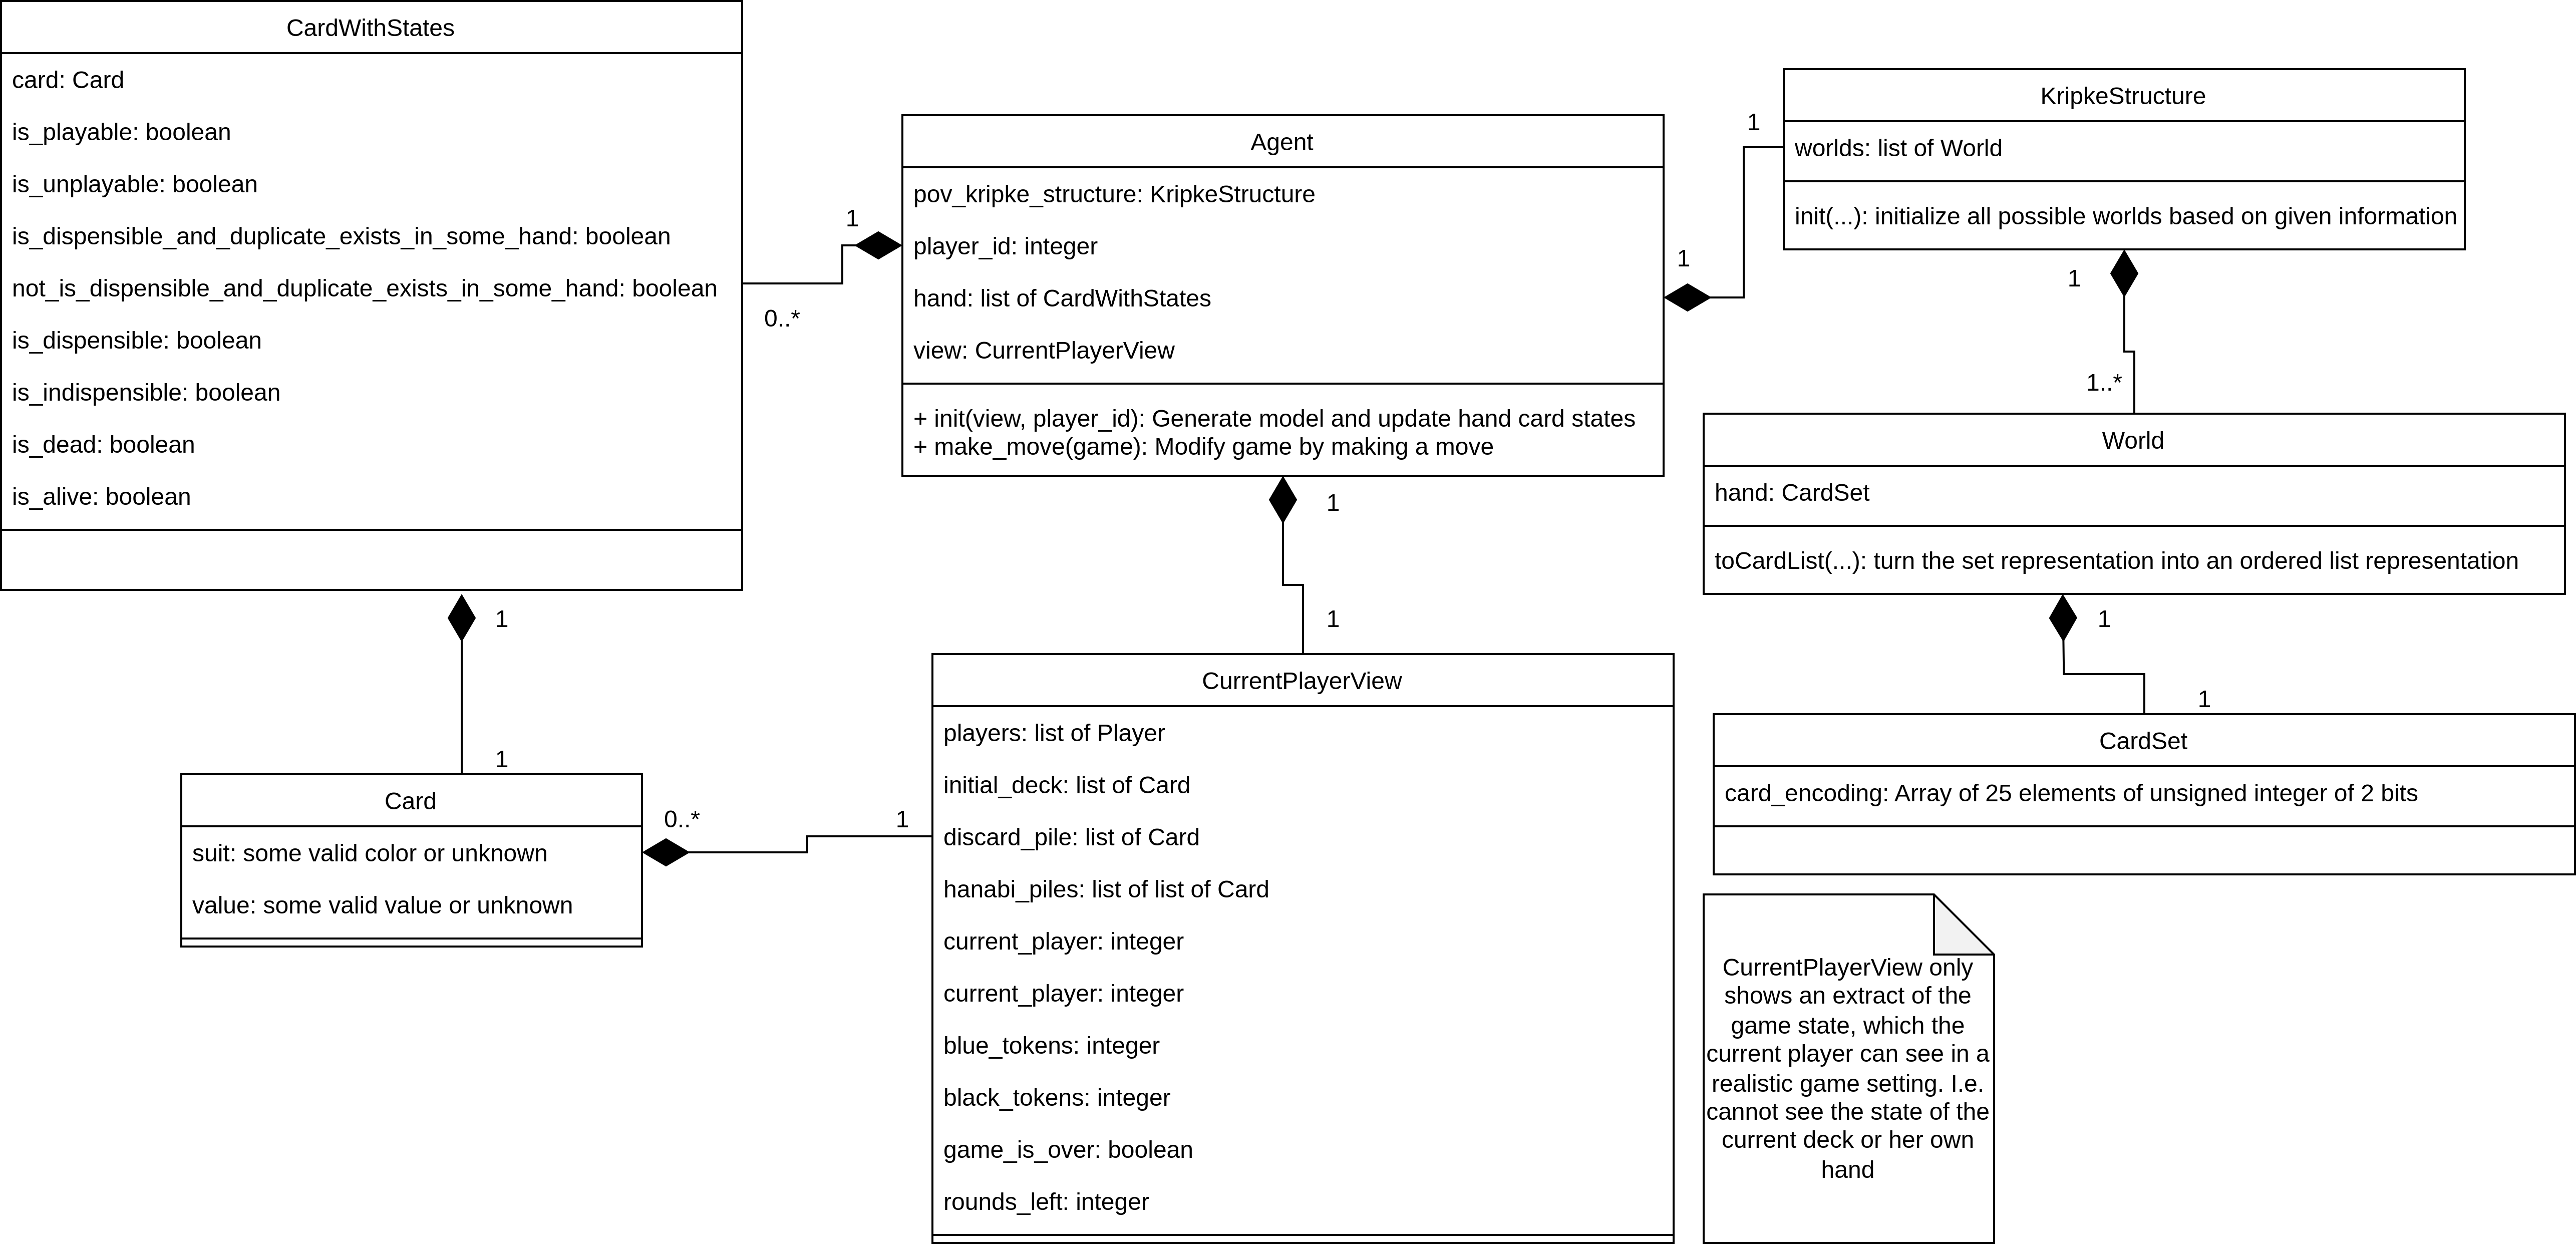
\includegraphics[width=22cm]{images/agent-uml-class-diagram.png}
	\caption{Low-fidelity class diagram for the things making up the Agent class}
	\label{fig:Agent-class-diagram}
\end{sidewaysfigure}

\subsection{Game simulation runner}
The glue-code between the Agents and the Game classes, is a class called SimulationRunner (defined in "{\tt src/ai\_simulation\_runner.zig}"), which takes a fully initialized Game and on-demand generates the agents and their epistemic models, and simulates a course of a game. See Figure \ref{fig:SimulationRunner-class-diagram} for the components making up the game simulator. The Game class has an element of randomness (in order to simulate random draws), so a seed can be provided when initializing the game in order to facilitate reproducibility.

\begin{figure}
	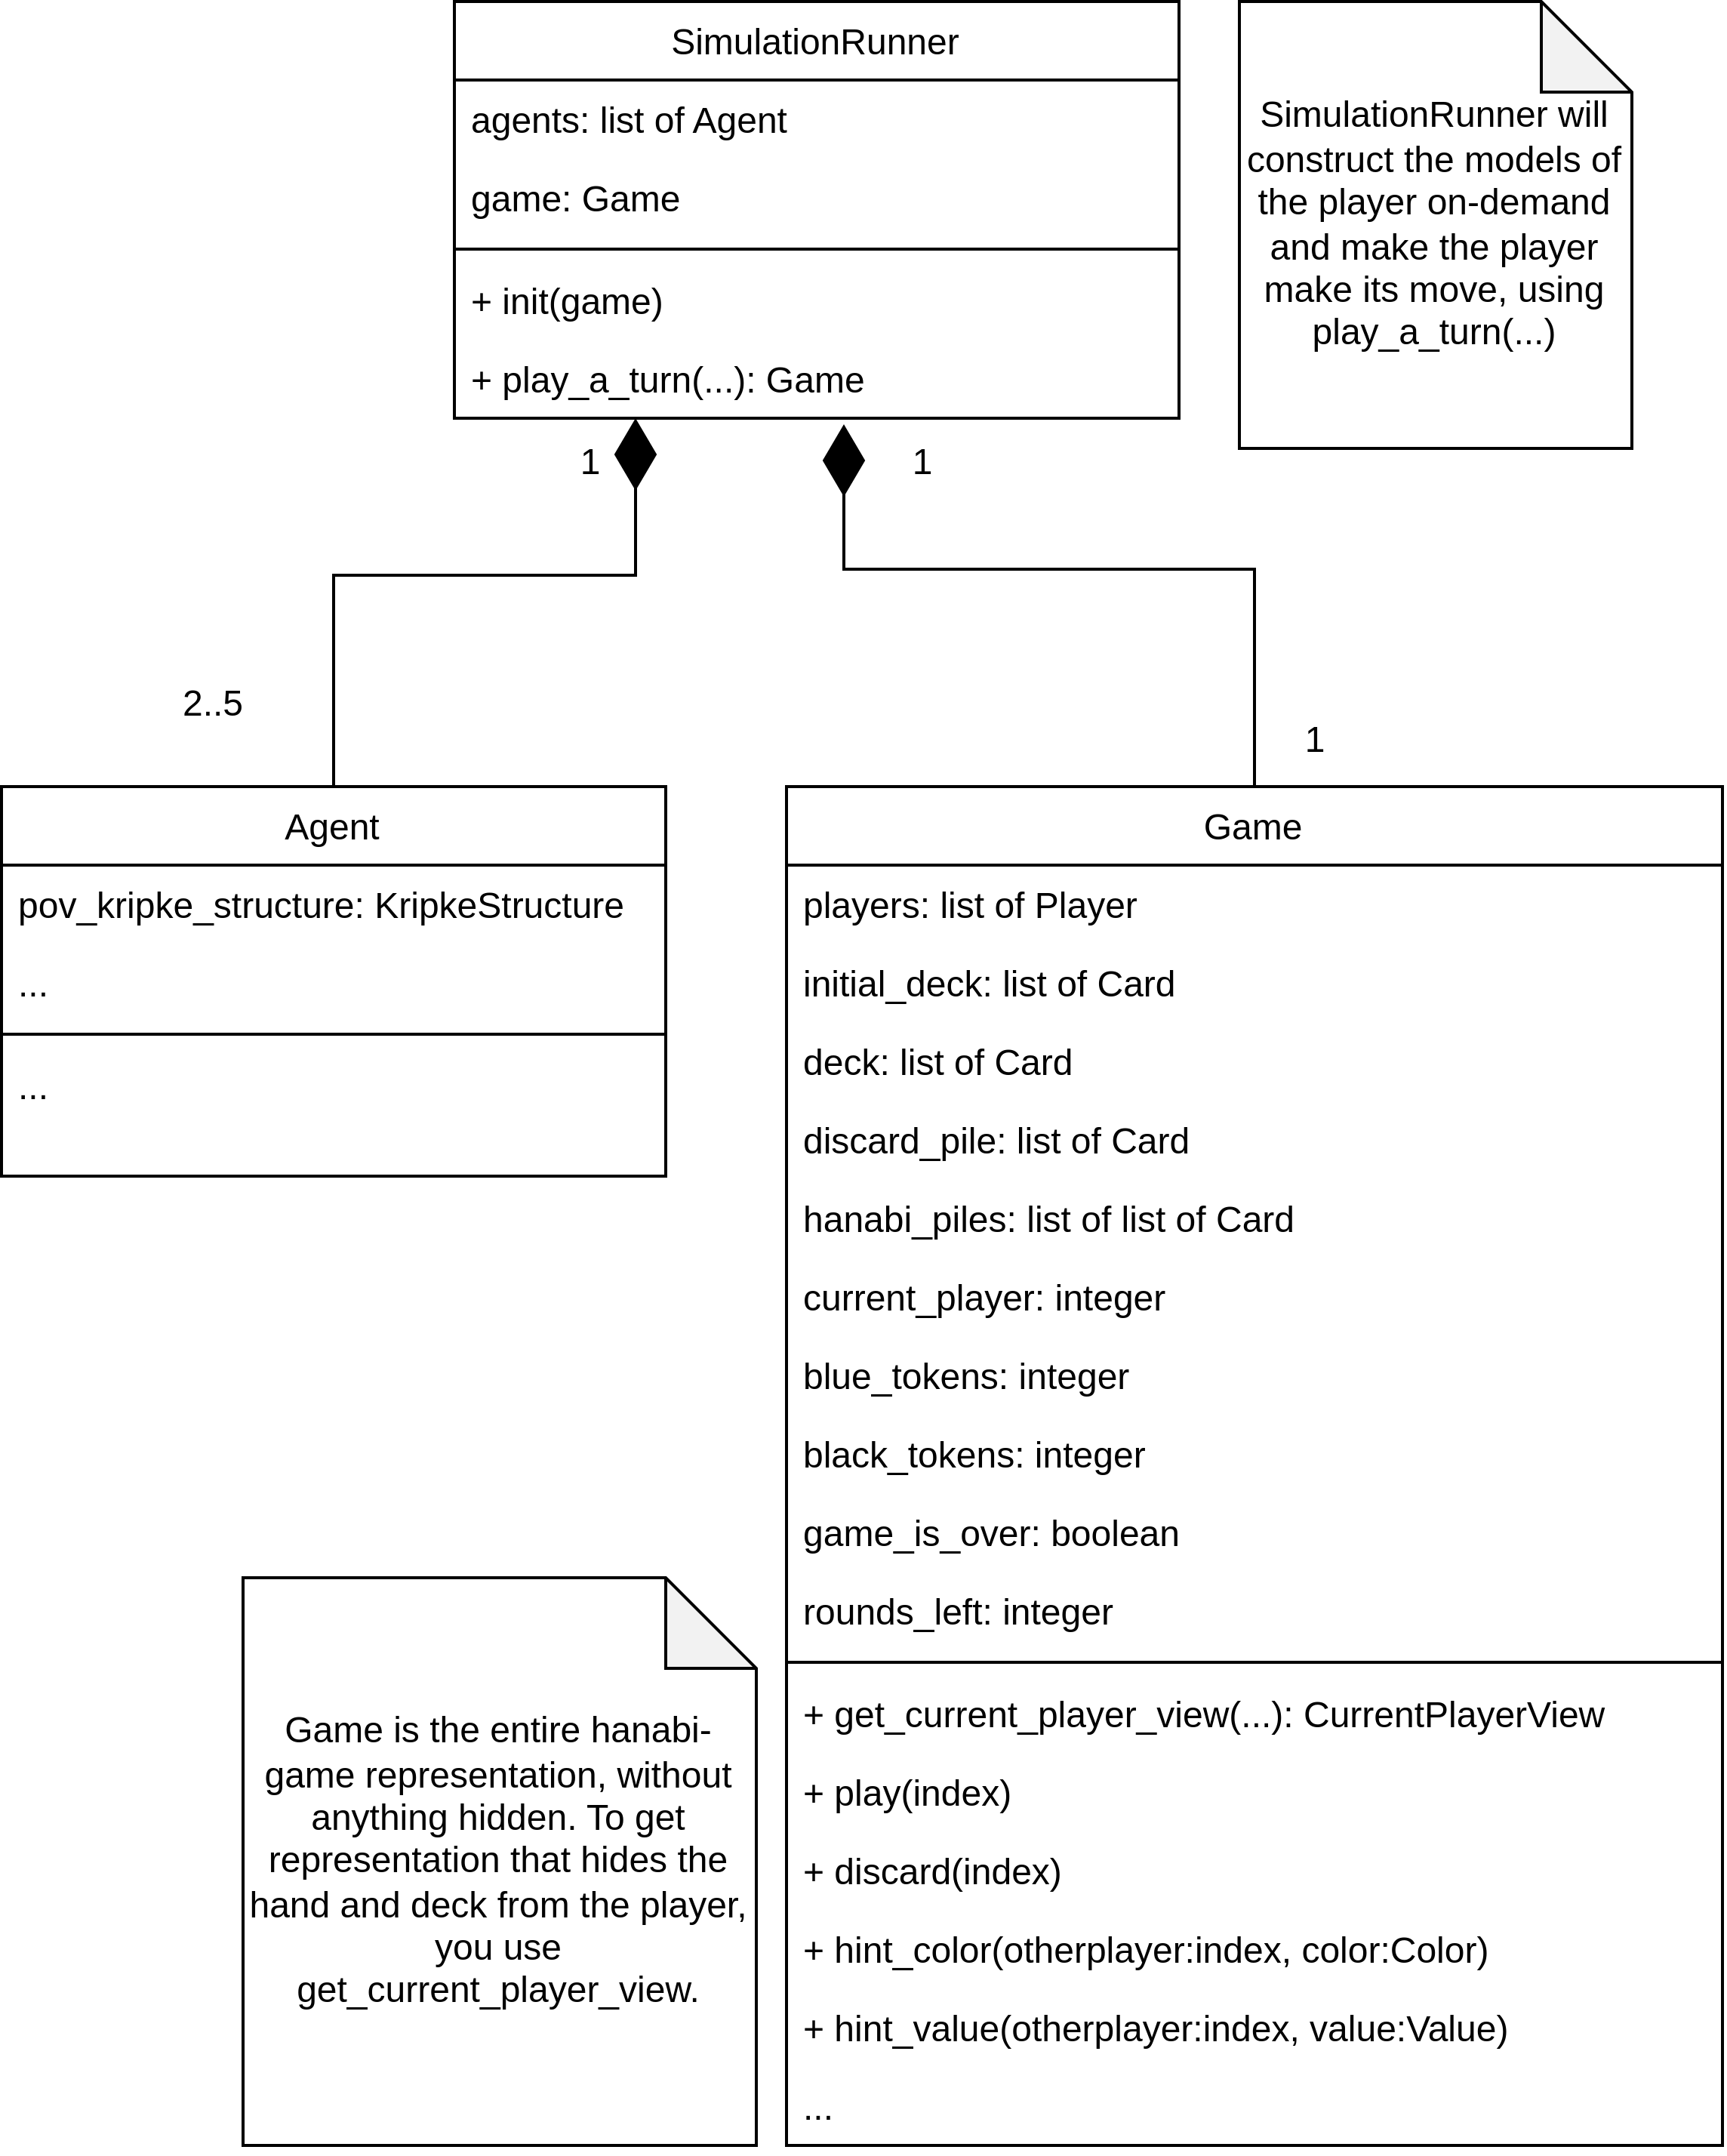
\includegraphics[width=13cm]{images/simulationrunner-uml-class-diagram.png}
	\caption{Low-fidelity class diagram for the things making up the SimulationRunner class}
	\label{fig:SimulationRunner-class-diagram}
\end{figure}

\section{Testing}
\ninanotes{
\begin{itemize}
\item Testing
\item Describe which kinds of tests are used and why.
\item Document the results.
\item Document whether (early) testing has lead to changes in design or
implementation.
\end{itemize}
}

\subsection{Testing my game implementation by making an interactive interface}

in {\tt src/cli\_simulation\_runner.zig} I made a made TUI application of the game, in order to inspect what would have if a specific action was executed, and whether it made sense. I guess it can be called a type of white box testing, since I am able to reproduce what happens if something fails.

\todo[inline]{Make the program have different compile arguments, in order to facilitate, like, how to run the runner? etc}
\todo[inline]{Make install instructions on zig so that the user can run my program.}

\subsection{Test system}
Making use of the fact that zig optimizes branches away, that it will know in compile-time will never run, I made an ad-hoc testing system. Because there were some things I would like to continually inspect. and Were hard to inspect without modifying the code. I.e. whiteboxtesting.

\section{Project management}

My main heuristic going into this project was to look for the minimal viable product, that made use of the theory of modal logic, and which was actually able to play Hanabi. So I tried to avoid premature optimizations in most places, except for parts I knew beforehand would be critical (like generating lots of possible worlds, and a compact representation for the worlds). 

I used git throughout the project as source-control, which also has the added benefit of keeping a log of the different commits, so that I could write notes there as I complete the product.


\section{Conclusion}
% \ninanotes{
% \begin{itemize}
% \item Conclusion
% \item What has been reached, how does the product work?
% \item What was not achieved or achieved exceeding the plan?
% \item Did you learn something new, techniques, socially?
% \item If there was more time . . .
% \item Personally, I . . . . . .
% \end{itemize}
% }

I have made a product based on a modified model of \SfiveN{}, denoted sub-\SfiveN{}, in which each agent can deduce a big set of possibilities for the other agents (and itself), and is able to look through each possible world to extract some property about each world.
The average score is 14.2 which is pretty far from many existing solutions.
The memory-layout of sub-\SfiveN{} in the case of Hanabi, is quite simple, given that it is implemented using a 3-dimensional array, and each world spends only 25 bytes of memory.
This compactness and good spatial locality is great for query algorithms that look through each world sequentially. 
Further space was saved by making sure that each world stores a multiset of cards, instead of a list of cards, while still retaining the ability to answer queries about specific cards on a agent's hand.

\subsection{Further work}
Public knowledge is very useful for strategies like the information strategy in \cite{CoxEtAl2015}, so 
if I had more time I would look into how public knowledge among the agents could be deduced from the sub-\SfiveN{} model, and whether it was actually possible to do this.
Furthermore, it would be interesting to see which strategies would work great in conjunction with the sub-\SfiveN{} model.
For instance the two rule-based strategies described in \cite{CoxEtAl2015}, I would argue, work completely orthogonally to the sub-\SfiveN{} model solution, which means that both of these strategies could be combined with sub-\SfiveN{} model in order to make better decisions.
In the case of the information strategy, the information gained by encoding the moves could further modify each agent's model and thereby gain more information by using such a strategy. 
Similarly, if the recommendation strategy says one of your cards is "playable" then you can eliminate all worlds for which that card is not playable.

Data representation and optimizing the Zig code would also be of priority if I had more time. An interesting option is to make a more in-depth comparison of the data-representations of the worlds described in section \ref{sec:representing-a-world}, and see how they would have affected performance in practice. Furthermore a lot of redundant permutations are generated whenever inspecting a possible world, which can be optimized away by only keep unique permutations.

Another interesting aspect of the Dynamic Epistemic Logic is to look into how a model could be viewed as a probabalistic model, rather than a certain knowledge model. 
For instance if a lot (but not all) of the possible worlds suggest that agent $p$'s 0th card is able to be played, then it is \emph{probably} able to be played.
\todo[inline]{look through for spent vs spend, what is the difference?}
\subsection{What I have learned}
In this project I learned a lot about modal logic, which strikes me as a good balance between using a powerful type of logic, as well as being pretty realistic to implement with reasonable performance, although, I have only scratched the surface of the subject, and there is a lot more to be explored in regards to it.

I also learned a lot about the programming language Zig, which has been a hobby-language of mine for quite a while, but I have not been able to test it on a project of this scale.
The main difficulty of using Zig is the fact that you have to take responsibility for how memory is managed. This can easily lead to decision-fatigue, especially if you are not accustomed to this style of programming.
\todo[inline]{find instances of zig and replace with Zig}
The advantage of Zig is that the language gives you a lot of tools in order to optimize code and data structures to a degree which is hard to do in a lot of languages.



% \oesuntaeoushnt
\bibliographystyle{plain}
\bibliography{bib.bib}
\appendix

\section{Generating the hanabi distinct combinations data and calculating mean, median and std} \label{appendix:python-distinct-combinations}
\begin{verbatim}
python version:
Python 3.11.2
packages version:
more-itertools==9.1.0
numpy==1.24.3
\end{verbatim}

\begin{lstlisting}[language=python]
import more_itertools
import random
import numpy
random.seed(0)

def main():
    
    # Blind draw 4 cards
    print("Blind draw 4 cards has:", 
    	getNumberOfCombinationsGivenHandOfSize(generateDeck(),4),
		"unique combinations")
    
    # Blind draw 5 cards
    print("Blind draw 5 cards has:", 
    	getNumberOfCombinationsGivenHandOfSize(generateDeck(),5),
		"unique combinations")
    
    # Random draw
    n = 30 #random rounds simulated
    # Data 2D array depending on how many players
    data = [[],[],[],[]]
    for _ in range(n):
        for player_count in range(2,6):
            number_of_cards = 5
            if(player_count >= 4):
                number_of_cards = 4
            deck = generateDeck()
            for _ in range((player_count-1)*number_of_cards):
                removeRandom(deck,random)
            data[player_count-2].append(
	   	 getNumberOfCombinationsGivenHandOfSize(deck,number_of_cards))
    
    p = 2
    for playerData in data:
        print("===number of players:",p)
        p+=1
        print("median:",numpy.median(playerData))
        print("mean:",numpy.mean(playerData))
        print("std:",numpy.std(playerData))
        print("min:",min(playerData))
        print("max:",max(playerData))

def generateDeck():
    arr = [1,1,1,2,2,3,3,4,4,5]
    superarr = []
    for i in range(5):
        for elem in arr:
                superarr.append(elem+10*i)
    return superarr

def removeRandom(deck, random):
    toRemove = random.randint(0,len(deck)-1)
    deck.pop(toRemove)

def getNumberOfCombinationsGivenHandOfSize(deck,size):
    return len(list(more_itertools.distinct_combinations(deck,size)))
main()
\end{lstlisting}

\end{document}
